% --- Contenuto LaTeX autogenerato da sezioneII.md (sezione 3) ---

\section{Giacinto Scelsi e il suo Metodo Compositivo}
\subsection{La crisi creativa}
Il metodo compositivo sviluppato da Scelsi dopo la crisi creativa dei primi anni Cinquanta rappresenta un unicum nel panorama della musica contemporanea. Come documentato da Bernardini e Pellegrini, Scelsi sviluppò una tecnica che consisteva nel registrare lunghe improvvisazioni pianistiche, inizialmente su dischi di cera e successivamente su nastro magnetico non appena la tecnologia divenne accessibile\cite[p. 176]{pro:beracpmm4ch2011}.

Questa metodologia nasceva dalla volontà di risolvere la dicotomia tra la spontaneità zen dell'improvvisazione e il lavoro meticoloso richiesto dalla notazione occidentale.
\subsection{L'ambiente di registrazione e le condizioni tecniche}
Le registrazioni di primaria importanza furono realizzate in ambiente domestico, con un approccio che privilegiava l'immediatezza della cattura sonora rispetto alla qualità tecnica. Come emerso dall'analisi delle registrazioni durante il laboratorio, Scelsi posizionava tipicamente il registratore vicino al divano, collocava il microfono sul divano stesso e si spostava al pianoforte posto a 3-4 metri di distanza, o alle ondiole.

Questa configurazione improvvisata, produceva registrazioni di qualità mediocre dal punto di vista tecnico, ma ricche di informazioni contestuali. Il riverbero naturale degli ambienti domestici, inizialmente percepito come difetto, si è rivelato un elemento distintivo che permette di identificare il luogo di registrazione: l'appartamento di Viale Mazzini 9 presenta caratteristiche acustiche diverse da quello di Via di Sant'Teodoro 8, dove Scelsi si trasferì successivamente.
\subsection{I trascrittori e il processo di mediazione}
Il sistema di lavoro di Scelsi prevedeva la collaborazione sistematica con trascrittori specializzati, compositori che traducevano le improvvisazioni registrate in notazione convenzionale.
\persona{Vieri Tosatti}{1920}{1999} fu il primo e più longevo trascrittore, responsabile della maggior parte delle partiture orchestrali e di opere significative come i Canti del Capricorno. La collaborazione con Tosatti fu facilitata dall'acquisto da parte di Scelsi di un registratore Revox A77 identico a quello del trascrittore, permettendo l'uso di riferimenti numerici precisi basati sul contatore della macchina. \persona{Sergio Cafaro}{1924}{2005} venne coinvolto specificamente per la trascrizione delle opere pianistiche, probabilmente in parallelo al lavoro di Tosatti. \persona{Enrico Filippini}{1932}{1988} subentrò quando Tosatti, afflitto da gravi problemi di vista, non poté più continuare la collaborazione. Filippini rappresenta l'ultimo anello di questa catena di mediazione tra l'improvvisazione e la partitura finale.

L'analisi delle annotazioni sulle scatole dei nastri ha rivelato un sofisticato sistema di comunicazione tra Scelsi e i suoi trascrittori. Le scatole riportano elenchi di numeri corrispondenti alle posizioni del contatore, accompagnati da indicazioni come ''buono per tromba'', ''buono per viola'', suggerendo che le composizioni venivano concepite come mosaici di frammenti da assemblare.

Questo metodo di lavoro è confermato dalla struttura stessa delle registrazioni. L'identificazione delle ''regioni'' durante la post-produzione - segmenti delimitati dai punti di start/stop del registratore - ha rivelato che alcuni nastri contengono oltre 60 frammenti distinti, mentre altri presentano registrazioni continue di diversi minuti\cite[p. 49]{bernardini_pellegrini_scelsi_2016}. La distribuzione statistica del numero di edits per nastro mostra una concentrazione nella fascia 7-10, con casi estremi che superano i 100 tagli, questi ultimi generalmente associati a materiali parlati piuttosto che musicali\cite[p. 49]{bernardini_pellegrini_scelsi_2016}.
\subsection{Gli strumenti della sperimentazione}
Oltre al pianoforte, strumento principale delle prime improvvisazioni, Scelsi integrò progressivamente nel suo arsenale strumentale due ondioline, sintetizzatori analogici che permettevano l'esplorazione microtonale\cite[p. 177]{bernardini_pellegrini_scelsi_2016}. L'analisi spettrale delle registrazioni con ondiola rivela l'uso sistematico di glissandi, battimenti e intervalli microtonali che sarebbero stati impossibili da realizzare su strumenti temperati.

I registratori utilizzati da Scelsi costituiscono essi stessi parte integrante del processo creativo. Il Revox G36, registratore a valvole ancora conservato presso la Fondazione, produce rumori meccanici caratteristici e vibrazioni delle valvole che sono entrati a far parte della ''firma sonora'' di molte registrazioni. Il successivo Revox A77, uno dei registratori a nastro più diffusi al mondo, garantiva maggiore stabilità e silenziosità operativa.

L'inventario delle macchine include anche un Tandberg, un Grundig e un Geloso, registratore italiano destinato principalmente alla dettatura. La presenza di nastri di formato ridotto compatibili solo con il Geloso conferma l'utilizzo di questa macchina, anche se l'apparecchio non è stato ritrovato nell'archivio.

\subsection{Le velocità di registrazione}

L'analisi delle velocità di registrazione utilizzate rivela scelte precise legate sia a considerazioni tecniche che estetiche. La velocità standard di 19 cm/s (7,5 pollici/secondo) predomina nelle registrazioni di lavoro. La velocità professionale di 38 cm/s (15 pollici/secondo), che garantisce maggiore risposta in frequenza e minor rumore di fondo, appare nelle registrazioni che Scelsi considerava particolarmente significative. La velocità ridotta di 9,5 cm/s (3,75 pollici/secondo) veniva impiegata per sessioni prolungate dove la durata prevaleva sulla qualità.

Particolarmente interessanti sono i nastri che presentano velocità variabili all'interno della stessa registrazione, evidenziando un uso creativo e non convenzionale del mezzo. Durante il laboratorio sono stati identificati nastri con cambi di velocità intenzionali, registrazioni sovrapposte a velocità diverse, esperimenti di feedback tra le piste.


\subsection{Gli strumenti a tastiera elettronici: pionierismo nella sintesi}
\begin{wrapfigure}{r}{0.4\textwidth} %this figure will be at the right
    \centering
    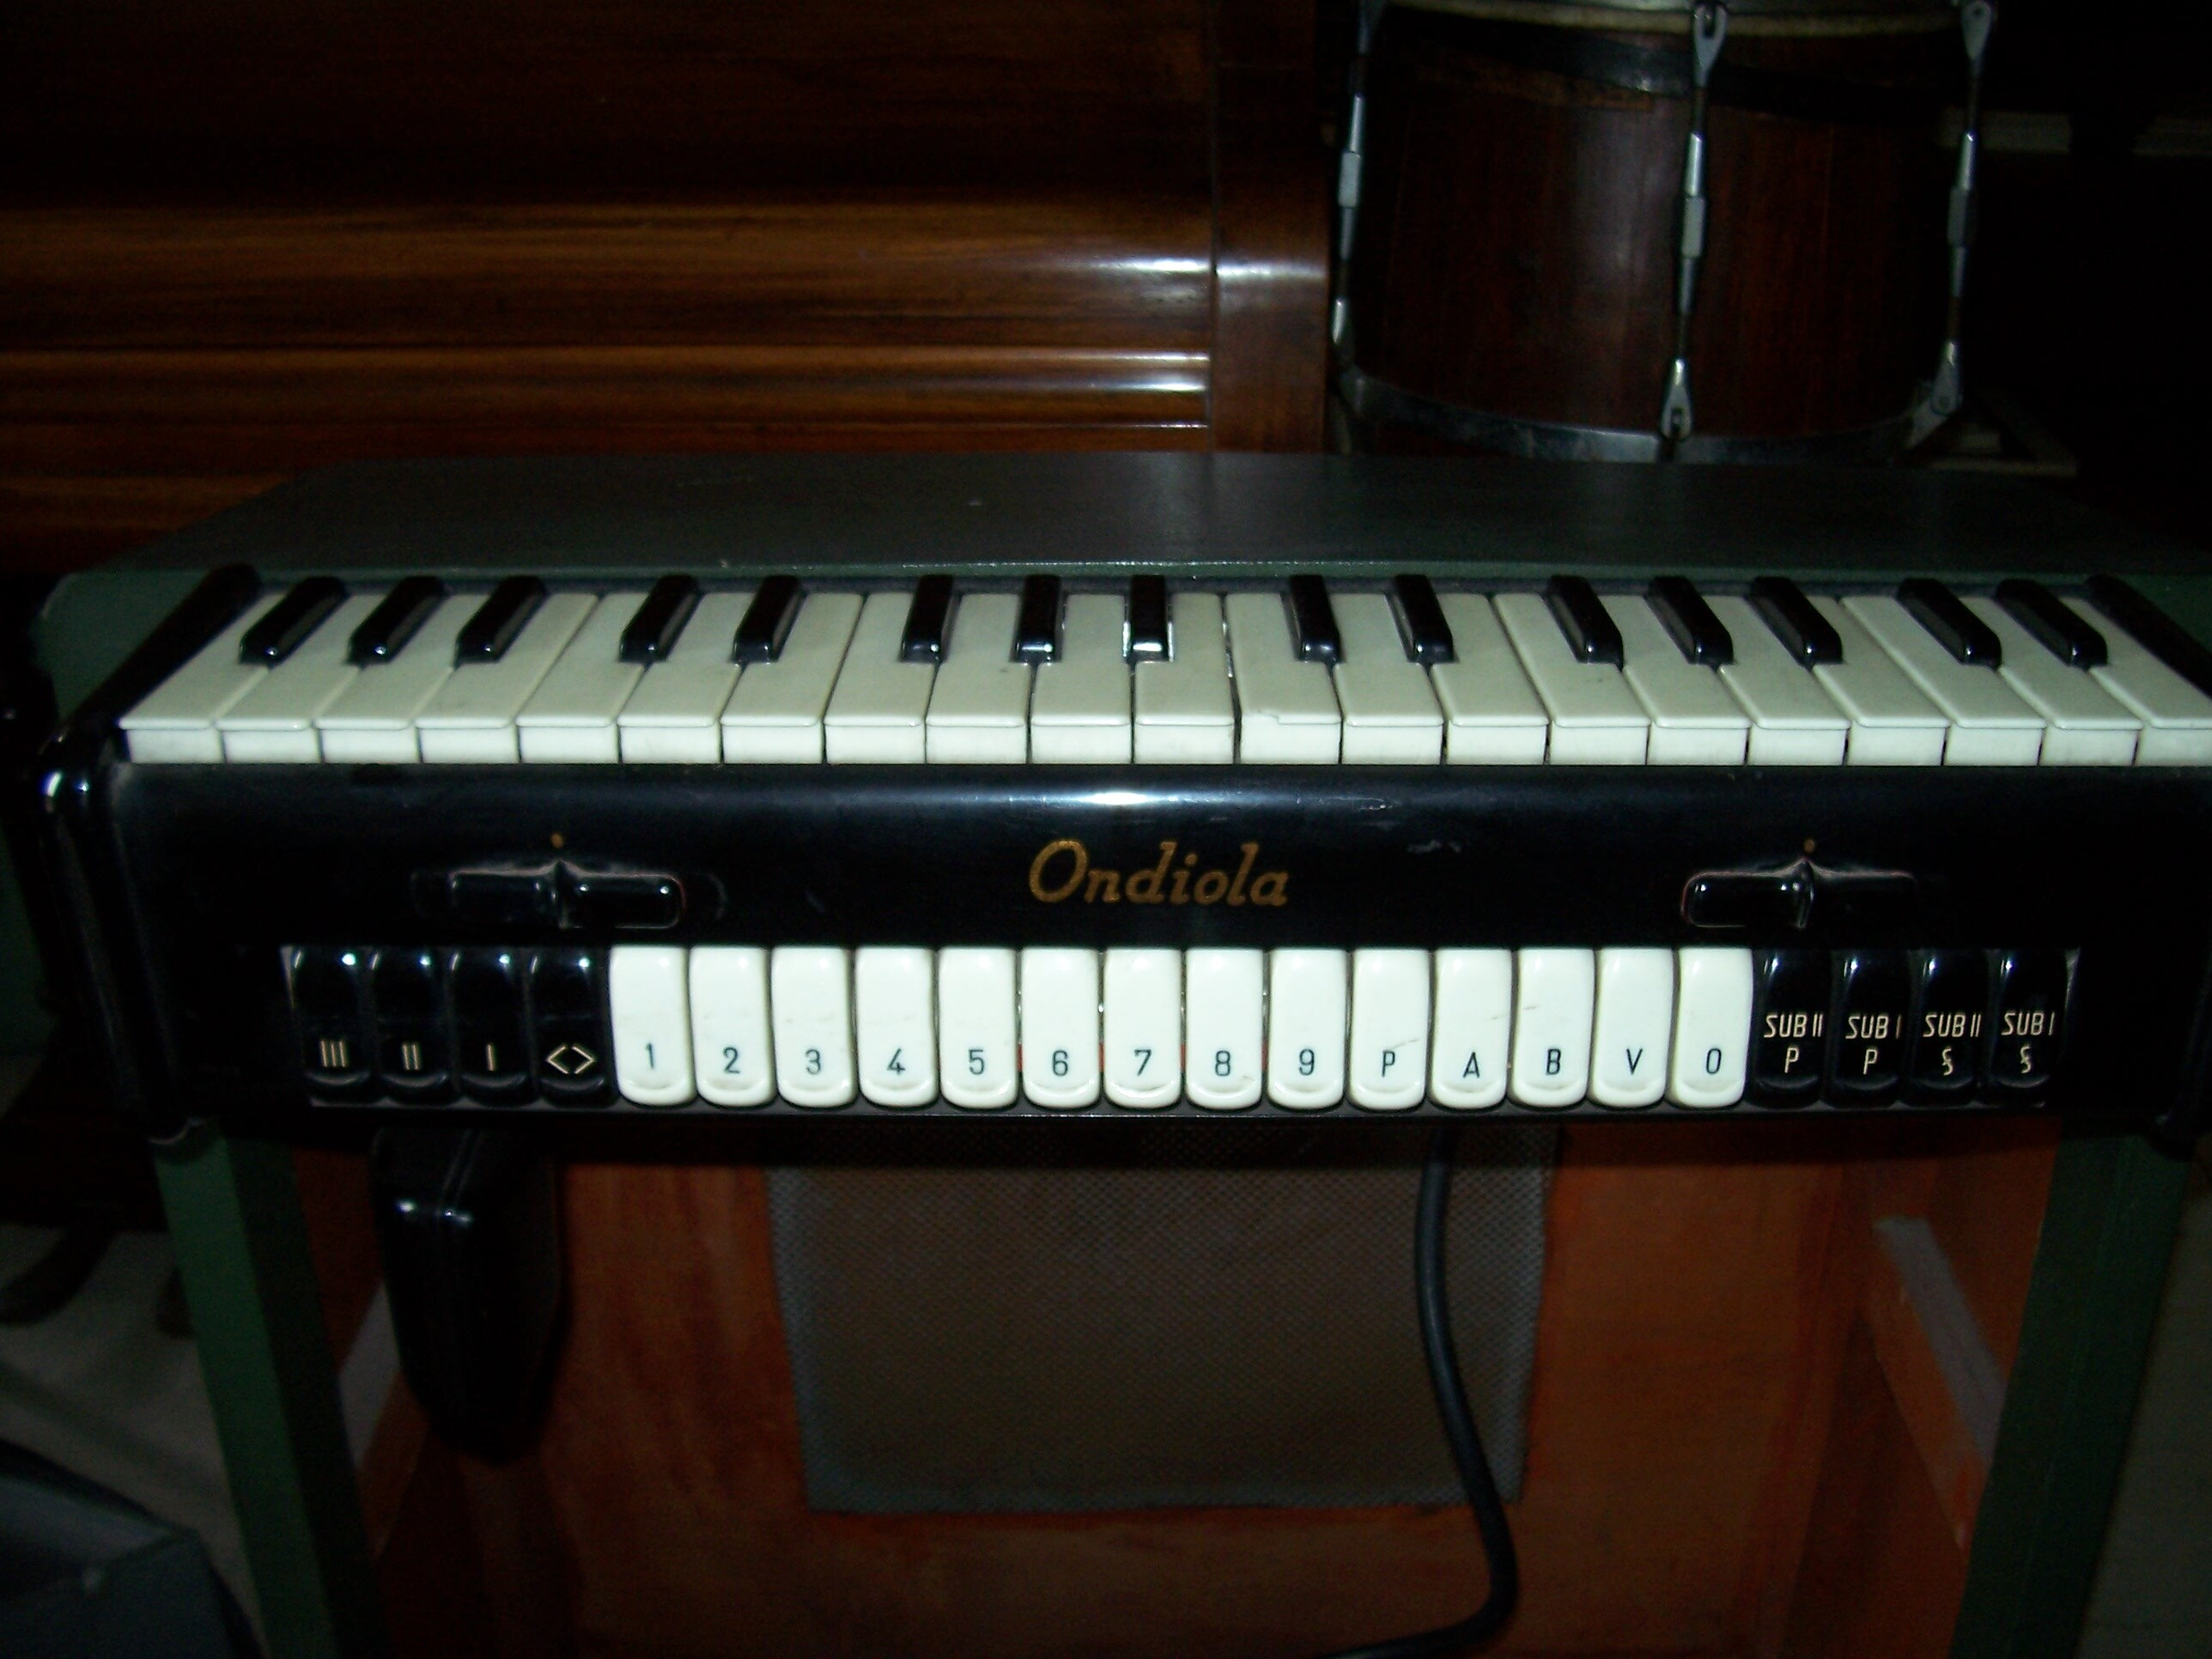
\includegraphics[width=0.4\textwidth]{docs/img/Ondiola_A-0062.jpg}
    \caption{L'Ondioline, strumento elettronico monofonico inventato da Georges Jenny.}
\end{wrapfigure}


L'introduzione di strumenti elettronici a tastiera nell'instrumentarium di Scelsi rappresenta un momento cruciale nell'evoluzione del suo linguaggio compositivo. In particolare, Scelsi utilizzò degli strumenti che, come emerso da recenti ritrovamenti d'archivio (cfr. Figura X e Y), erano copie italiane delle Clavioline Selmer, prodotte dalla Elettronica Musicale Italiana (EMI) e commercializzate con il nome "Ondiola" (da non confondere con le omonime Ondioline inventate da \persona{Georges Marcel Charles Jenny}{1913}{1975}, che ebbero una diffusione più limitata). Questi sintetizzatori analogici monofonici permettevano la generazione di forme d'onda con possibilità di controllo timbrico e, in alcuni modelli, di effetti come il vibrato e il glissando, offrendo nuove vie per l'esplorazione sonora, inclusa quella microtonale attraverso la prassi esecutiva.
L'analisi spettrale delle registrazioni effettuate con questi strumenti, condotta durante il laboratorio utilizzando software di analisi audio contemporanei, ha rivelato l'uso sistematico di tecniche compositive innovative: Glissandi microtonali continui, impossibili da realizzare su strumenti acustici tradizionali, che creano traiettorie sonore fluide attraverso lo spazio delle altezze; Battimenti controllati attraverso la sovrapposizione di frequenze vicine.